\chapter{PDZ}
\label{chap:PDZ}

    \clearpage

\paragraph{Alignements Blast croisés}


    \begin{table}[!htbp]
      \centering

      \begin{tabular}{ccccccccc}

        \toprule
        Protein & 1G9O & 1IHJ & 1N7E & 1R6J & 2BYG & 3K82 & CASK & TIAM1 \\
        \cmidrule{1-9}

        1G9O &  2e-66 & 5e-10 &  0.002 & 3e-07 & 2e-11 & 1e-12 & 5e-05 & 9e-07 \\     
        1IHJ &  5e-10 & 3e-68 &  2e-07 & no &   2e-08 & 9e-14 & 4e-06 & no    \\
        1N7E &  0.002 & 2e-07 &  3e-67 & no &    3e-14 & 2e-10 & 9e-12 & 5e-05 \\
        1R6J &  3e-07 & no  &    no  &  1e-59 &  no &   1e-06 & 0.007 & no    \\
        2BYG &  2e-11 & 2e-08 &  3e-14 & no &    7e-71 & 3e-15 & 2e-07 & 5e-05 \\
        3K82 &  1e-12 & 9e-14 &  2e-10 & 1e-06 & 3e-15 & 4e-70 & 1e-07 & 6e-04 \\
        CASK &  5e-05 & 4e-06 &  9e-12 & 0.007 & 2e-07 & 1e-07 & 7e-61 & 5e-04 \\
        TIAM1 & 9e-07 &  no &    5e-05 & no  &   5e-05 & 6e-04 & 5e-04 & 1e-68 \\
        \bottomrule


      \end{tabular}      
      \caption{E-value des alignements Blast native vs native pour nos séquences PDZ. (no= pas de touche avec une E-value inférieure à 10)}
\label{tab:Xblast}      
    \end{table}


requête sur le site d'uniprot

Target database uniprot (swissprot + trEMBL)

Matrix BLOSUM62

Filtering NO

Gapped YES


Puis selection à la main -->
enveler les redondances flagrantes
 + avoir un compromis entre diversité et qualité de l'alignement
 + rester dans la zone de ce qui a déjà été fait.



    \begin{table}[!htbp]
      \centering

      \begin{tabular}{cccc}

        \toprule
        protéines & seq NB & E value seuil & \% identité \\
        \cmidrule{1-4}
     1G9O  & 63  &    10-32  &  95-67 \\
     1IHJ  & 56  &    10-10  &  95-38 \\
     1N7E  & 93  &    10-45  &  95-84 \\
     1R6J  & 86  &    10-43  &  95-85 \\
     2BYG  & 82  &    10-41  &  95-78 \\
     3K82  & 88  &    10-46  &  95-81 \\


        \bottomrule


      \end{tabular}      
      \caption{Sélection des homologues.}
\label{tab:freq_AA_ALL}      
    \end{table}



    \clearpage

\paragraph{Fréquences des acides aminés}


    \begin{table}[!htbp]
      \centering

      \begin{tabular}{ccc}

        \toprule
        Groupe & acides aminés & propriétés\\
        \cmidrule{1-3}

        1   & Ala,Cys,Thr & petit\\
        2   & Ser &\\
        \cmidrule{1-3}
        3   & Glu,Asp & chargé négativement\\
        \cmidrule{1-3}
        4   & Gln,Asn & polaire\\
        \cmidrule{1-3}
        5   & Ile,Leu,Val & apolaire\\
        \cmidrule{1-3}
        6   & Met & non polaire\\
        \cmidrule{1-3}
        7   & Hip,Hid,Hie & chargé positivement\\
        8   & Arg \\
        9   & Lys \\
        \cmidrule{1-3}
        10  & Phe,Trp & aromatique\\
        11  & Tyr \\
        \cmidrule{1-3}
        12  & Gly,Pro & non mutable\\
        \bottomrule


      \end{tabular}      
      \caption{Les groupes d'acides aminés utilisés pour l'optimisation des énergies de références.}
\label{tab:AA_groupes}      
    \end{table}



    \begin{table}[!htbp]
      \centering

      \begin{tabular}{cc}

        \toprule
        acides aminés & fréquence \\
        \cmidrule{1-2}

        Ala &   0.090 \\      
        Cys &   0.028 \\  
        Thr &   0.060 \\  
        Ser &   0.071 \\  
        Glu &   0.062 \\  
        Asp &   0.044 \\  
        Gln &   0.039 \\  
        Asn &   0.055 \\  
        Ile &   0.046 \\  
        Leu &   0.075 \\  
        Val &   0.069 \\  
        Met &   0.017 \\  
        His &   0.021 \\  
        Arg &   0.047 \\  
        Lys &   0.070 \\  
        Phe &   0.035 \\  
        Trp &   0.011 \\  
        Tyr &   0.035 \\  
        Gly &   0.075 \\  
        Pro &   0.046 \\      
        \bottomrule


      \end{tabular}      
      \caption{Fréquences des acides aminés d'après dans les  protéines.}
\label{tab:AA_groupes}      
    \end{table}


    \begin{table}[!htbp]
      \centering

      \begin{tabular}{c|cc|cc}

        \toprule
        acides aminés & résidus enfouis & groupe & résidus exposés & groupe\\
        \cmidrule{1-5}

        Ala &         0.068 &       &   0.048   \\
        Cys &         0.016 &  0.147  &   0.004 & 0.135  \\    
        Thr &         0.062 &        &   0.081   \\
        \cmidrule{1-5}
        Ser &        \multicolumn{2}{c|}{0.067}     &   \multicolumn{2}{c}{0.066}  \\
        \cmidrule{1-5}
        Glu &         0.053 & 0.089        &   0.078 & 0.134 \\
        Asp &         0.035 &    &   0.055   \\
        \cmidrule{1-5}
        Gln &         0.022 & 0.051 &   0.052 & 0.117\\
        Asn &         0.028 &         &   0.064   \\
        \cmidrule{1-5}
        Ile &         0.136 & 0.362        &   0.071  \\
        Leu &         0.120 &   &   0.055 & 0.192 \\
        Val &         0.105 &         &   0.065  \\
        \cmidrule{1-5}
        Met &    \multicolumn{2}{c|}{0.027}      &  \multicolumn{2}{c}{0.018} \\
        \cmidrule{1-5}
        Hip &         0.022 &      &   0.041 \\
        Hid &         0     &  0.022 &   0    & 0.041\\
        Hie &         0     &        &   0     \\
        \cmidrule{1-5}
        Arg &        \multicolumn{2}{c|}{0.037}      &  \multicolumn{2}{c}{0.059}\\
        \cmidrule{1-5}
        Lys &        \multicolumn{2}{c|}{0.058}         &  \multicolumn{2}{c}{0.079} \\
        \cmidrule{1-5}
        Phe &         0.037 &  0.037  &   0.017 & 0.017 \\
        Trp &         0.0   &        &   0.0  \\
        \cmidrule{1-5}
        Tyr &       \multicolumn{2}{c|}{0.008}      &  \multicolumn{2}{c}{0.015}\\
        \cmidrule{1-5}
        Gly &         0.070  & 0.089 &   0.088 & 0.123\\
        Pro &         0.019  &        &   0.035  \\
        \bottomrule


      \end{tabular}      
      \caption{Les groupes d'acides aminés utilisés pour l'optimisation des énergies de références.}
\label{tab:AA_groupes}      
    \end{table}




    \begin{table}[!htbp]
      \centering

      \begin{tabular}{ccccccccc}

        \toprule
        aa & 3K82 & 2BYG & 1R6J & 1N7E & 1IHJ & 1G9O & cask & tiam1 \\
        \cmidrule{1-9}
     ALA  & 0.045  &     0.077   &    0.085   &    0.071   &    0.100   &    0.067   &    0.046  &     0.071  \\
     CYS  & 0.021  &     0.012   &    0.027   &    0.000   &    0.011   &    0.018   &    0.030  &     0.000  \\
     THR  & 0.119  &     0.056   &    0.089   &    0.070   &    0.020   &    0.032   &    0.044  &     0.030  \\
        \cmidrule{1-9}
     SER  & 0.083  &     0.073   &    0.077   &    0.079   &    0.082   &    0.046   &    0.044  &     0.048  \\
        \cmidrule{1-9}
     GLU  & 0.039  &     0.048   &    0.001   &    0.078   &    0.010   &    0.129   &    0.063  &     0.059  \\
     ASP  & 0.047  &     0.076   &    0.000   &    0.026   &    0.028   &    0.024   &    0.039  &     0.030  \\
        \cmidrule{1-9}
     ASN  & 0.062  &     0.054   &    0.048   &    0.001   &    0.004   &    0.017   &    0.007  &     0.029  \\
     GLN  & 0.021  &     0.050   &    0.000   &    0.032   &    0.027   &    0.023   &    0.014  &     0.001  \\
        \cmidrule{1-9}
     ILE  & 0.120  &     0.102   &    0.219   &    0.084   &    0.193   &    0.030   &    0.197  &     0.116  \\
     VAL  & 0.073  &     0.108   &    0.110   &    0.041   &    0.149   &    0.119   &    0.138  &     0.131  \\
     LEU  & 0.063  &     0.099   &    0.087   &    0.131   &    0.118   &    0.114   &    0.151  &     0.255  \\
        \cmidrule{1-9}
     MET  & 0.020  &     0.000   &    0.027   &    0.020   &    0.010   &    0.008   &    0.084  &     0.015  \\
        \cmidrule{1-9}
     HID  & 0.000  &     0.000   &    0.000   &    0.000   &    0.000   &    0.000   &    0.000  &     0.000  \\
     HIE  & 0.000  &     0.000   &    0.000   &    0.000   &    0.000   &    0.000   &    0.000  &     0.000  \\
     HIP  & 0.025  &     0.025   &    0.032   &    0.026   &    0.004   &    0.043   &    0.012  &     0.001  \\
        \cmidrule{1-9}
     ARG  & 0.063  &     0.012   &    0.000   &    0.047   &    0.060   &    0.106   &    0.006  &     0.029  \\
        \cmidrule{1-9}
     LYS  & 0.042  &     0.087   &    0.055   &    0.077   &    0.015   &    0.036   &    0.071  &     0.058  \\
     TRP  & 0.000  &     0.000   &    0.000   &    0.000   &    0.000   &    0.000   &    0.000  &     0.000  \\
     PHE  & 0.063  &     0.000   &    0.055   &    0.000   &    0.061   &    0.039   &    0.039  &     0.059  \\
        \cmidrule{1-9}
     TYR  & 0.000  &     0.025   &    0.000   &    0.000   &    0.003   &    0.004   &    0.000  &     0.057  \\
     GLY  & 0.062  &     0.088   &    0.080   &    0.157   &    0.065   &    0.095   &    0.000  &     0.000  \\
     PRO  & 0.021  &     0.000   &    0.000   &    0.052   &    0.032   &    0.039   &    0.006  &     0.000  \\


        \bottomrule


      \end{tabular}      
      \caption{Compositions en acides aminés des séquences expérimentales homologues aux positions enfouies et actives.}
\label{tab:freq_AA_ALL}      
    \end{table}

    \begin{table}[!htbp]
      \centering

      \begin{tabular}{ccccccccc}

        \toprule
        aa & 3K82 & 2BYG & 1R6J & 1N7E & 1IHJ & 1G9O & cask & tiam1 \\
        \cmidrule{1-9}

   ALA  & 0.056  &  0.076  &   0.039  &   0.055  &   0.020 &   0.061  &   0.019  &   0.073 \\                                         
   CYS  & 0.000  &  0.000  &   0.000  &   0.000  &   0.011 &   0.012  &   0.000  &   0.022 \\                                           
   THR  & 0.122  &  0.058  &   0.100  &   0.104  &   0.069 &   0.028  &   0.080  &   0.073 \\                                        
        \cmidrule{1-9}
   SER  & 0.076  &  0.029  &   0.080  &   0.049  &   0.072 &   0.050  &   0.053  &   0.151 \\                                          
        \cmidrule{1-9}
   GLU  & 0.025  &  0.063  &   0.061  &   0.092  &   0.081 &   0.081  &   0.099  &   0.113 \\                                           
   ASP  & 0.074  &  0.035  &   0.093  &   0.018  &   0.082 &   0.046  &   0.041  &   0.084 \\                                           
        \cmidrule{1-9}
   ASN  & 0.045  &  0.075  &   0.078  &   0.030  &   0.096 &   0.048  &   0.088  &   0.060 \\                                         
   GLN  & 0.027  &  0.012  &   0.046  &   0.035  &   0.031 &   0.061  &   0.125  &   0.051 \\                                            
        \cmidrule{1-9}
   ILE  & 0.143  &  0.057  &   0.057  &   0.151  &   0.026 &   0.022  &   0.035  &   0.048 \\                                               
   VAL  & 0.056  &  0.104  &   0.043  &   0.053  &   0.068 &   0.088  &   0.074  &   0.037 \\                                        
   LEU  & 0.025  &  0.074  &   0.022  &   0.093  &   0.034 &   0.087  &   0.040  &   0.056 \\                                          
        \cmidrule{1-9}
   MET  & 0.049  &  0.025  &   0.021  &   0.000  &   0.015 &   0.007  &   0.028  &   0.001 \\                                          
        \cmidrule{1-9}
   HID  & 0.000  &  0.000  &   0.000  &   0.000  &   0.000 &   0.000  &   0.000  &   0.000 \\                                         
   HIE  & 0.000  &  0.000  &   0.000  &   0.000  &   0.000 &   0.000  &   0.000  &   0.000 \\                                         
   HIP  & 0.050  &  0.038  &   0.044  &   0.016  &   0.029 &   0.041  &   0.081  &   0.013 \\                                        
        \cmidrule{1-9}
   ARG  & 0.024  &  0.012  &   0.066  &   0.040  &   0.060 &   0.070  &   0.119  &   0.059 \\                                          
        \cmidrule{1-9}
   LYS  & 0.074  &  0.063  &   0.066  &   0.072  &   0.103 &   0.070  &   0.084  &   0.110 \\                                          
        \cmidrule{1-9}
   TRP  & 0.000  &  0.000  &   0.000  &   0.000  &   0.000 &   0.000  &   0.000  &   0.000 \\                                         
        \cmidrule{1-9}
   PHE  & 0.022  &  0.037  &   0.030  &   0.018  &   0.005 &   0.011  &   0.006  &   0.001 \\                                         
        \cmidrule{1-9}
   TYR  & 0.000  &  0.035  &   0.000  &   0.037  &   0.003 &   0.021  &   0.001  &   0.015 \\
        \cmidrule{1-9}
   GLY  & 0.100  &  0.149  &   0.089  &   0.093  &   0.130 &   0.130  &   0.015  &   0.019 \\                                            
   PRO  & 0.025  &  0.050  &   0.054  &   0.037  &   0.055 &   0.054  &   0.002  &   0.005 \\                                         
        \bottomrule


      \end{tabular}      
      \caption{Compositions en acides aminés des séquences expérimentales homologues aux positions exposées et actives.}
\label{tab:freq_AA_ALL}      
    \end{table}


    \clearpage
   \paragraph{Résultats Superfamily}



    \begin{table}[h]
           \raggedleft{}

      \begin{tabular}{cccccc}

        \toprule
        Protein & Match/seq & Superfamily & Superfamily & Family & Family \\
                & size      & Evalue      & success     & Evalue & success\\
        \cmidrule{1-6}
        1G9O  & 77/91 &  3.8e-9  & 10000 & 3.8e-3 & 10000 \\
        1IHJ  & 84/94 &  9.8e-4  &  9997 & 2.4e-3 &  9997 \\
        1N7E  & 79/95 &  3.9e-7  & 10000 & 2.3e-3 & 10000 \\
        1R6J  & 61/82 &  1.4e-1  &  8855 & 1.2e-2 &  8855 \\
        2BYG  & 58/97 &  4.7e-2  &  9956 & 7.6e-3 &  9956 \\
        3K82  & 84/97 & 1.4e-12  & 10000 & 2.6e-3 & 10000 \\
        CASK  & 42/83 &  7.7e-1  &   654 & 2.6e-2 &   654 \\
        TIAM1 & 46/94 &     1.8  &   109 & 2.5e-2 &   109 \\
        \bottomrule        
      \end{tabular}   
     \caption{Résultats Superfamily pour les séquences Proteus des  protéines PDZ}   
\label{tab:superfamily_bestRE}       
\end{table}




    \begin{table}[h]
           \raggedleft{}

      \begin{tabular}{cccccc}

        \toprule
        Protein & Match/seq & Superfamily & Superfamily & Family & Family \\
                & size      & Evalue      & success     & Evalue & success\\
        \cmidrule{1-6}
        1G9O  & /91 &  &  &  &  \\
        1IHJ  & /94 &  &  &  &  \\
        1N7E  & /95 &  &  &  &  \\
        1R6J  & /82 &  &  &  &  \\
        2BYG  & /97 &  &  &  &  \\
        3K82  & /97 &  &  &  &  \\
        CASK  & /83 &  &  &  &  \\
        TIAM1 & /94 &  &  &  &  \\
        \bottomrule        
      \end{tabular}   
     \caption{Résultats Superfamily pour les séquences Rosetta des  protéines PDZ}   
\label{tab:superfamily_bestRE}       
\end{table}




   \begin{figure}[t]
     \centering
     \begin{tabular}{cc}
       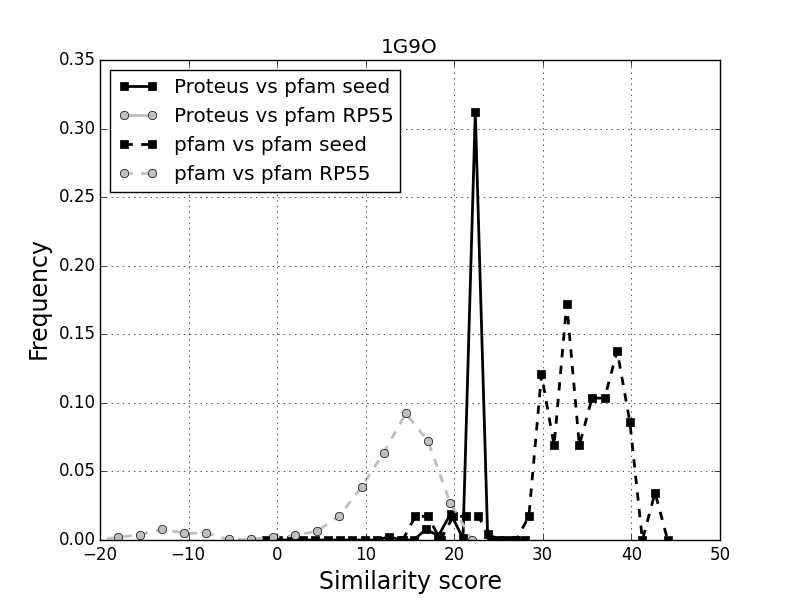
\includegraphics[width=8.45cm]{1G9O_simil_byseq.png} &
       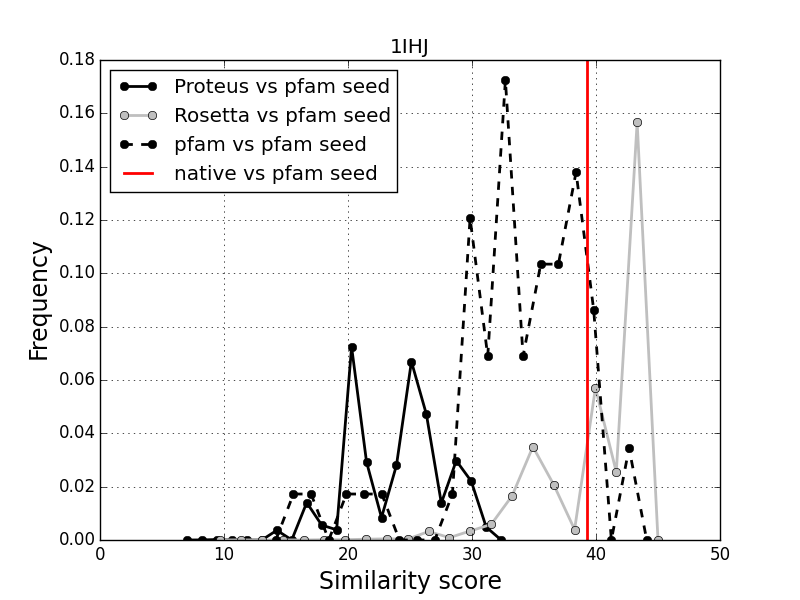
\includegraphics[width=8.45cm]{1IHJ_simil_byseq.png} \\
       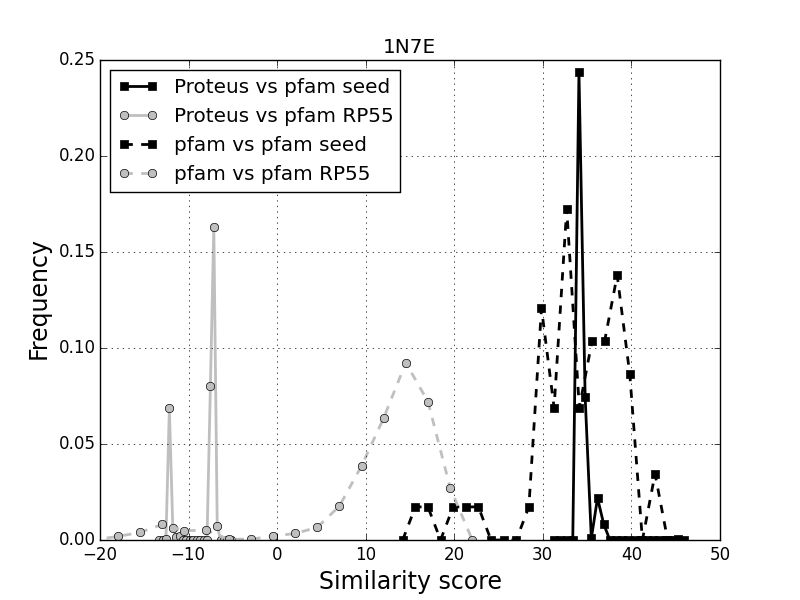
\includegraphics[width=8.45cm]{1N7E_simil_byseq.png} &
       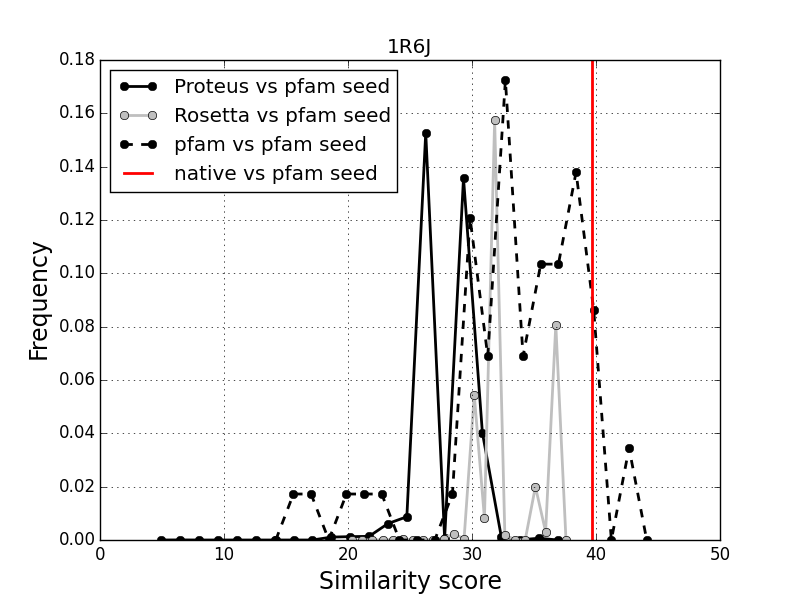
\includegraphics[width=8.45cm]{1R6J_simil_byseq.png} \\
       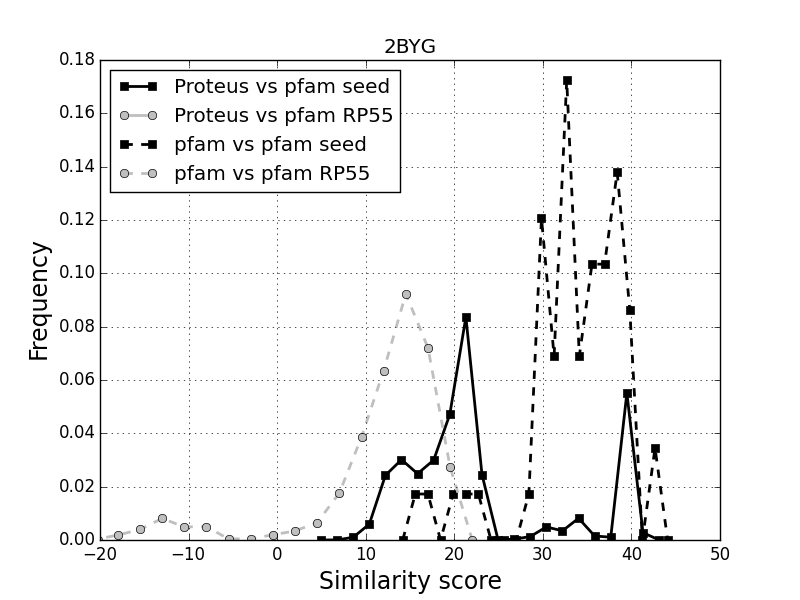
\includegraphics[width=8.45cm]{2BYG_simil_byseq.png} &
       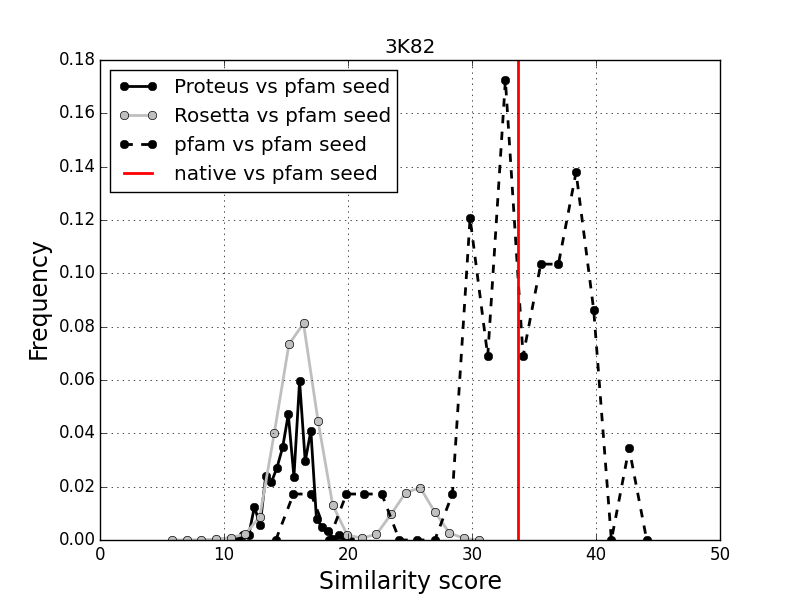
\includegraphics[width=8.45cm]{3K82_simil_byseq.png} \\ 
       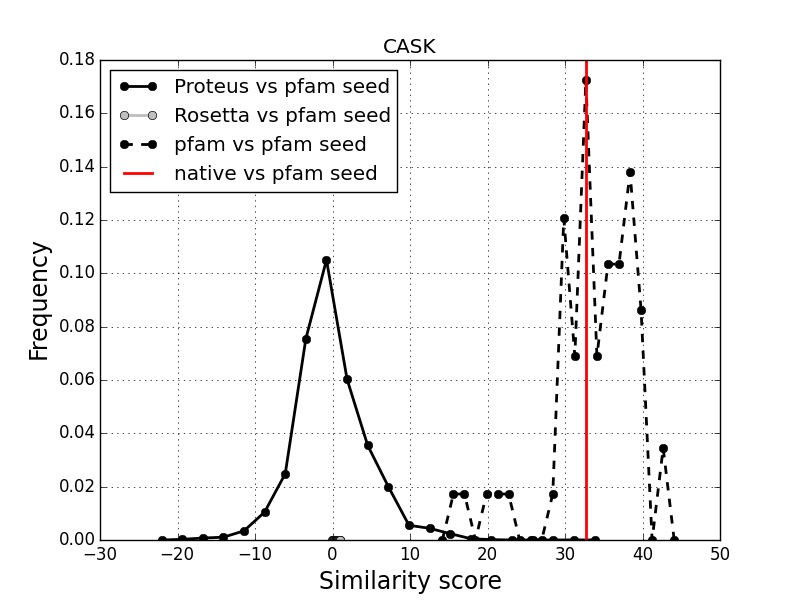
\includegraphics[width=8.45cm]{CASK_simil_byseq.png} &
       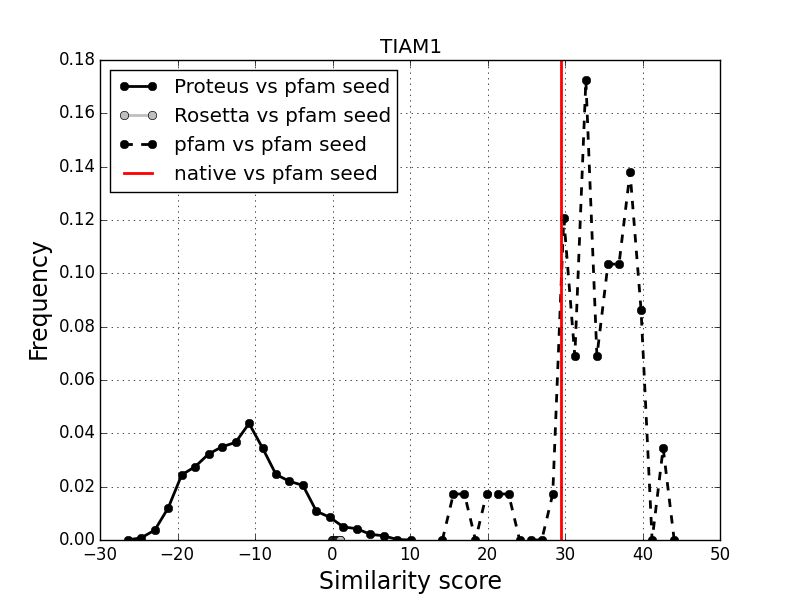
\includegraphics[width=8.45cm]{TIAM1_simil_byseq.png} \\ 

     \end{tabular}
     \caption{Similarité par séquence pour les séquences Proteus des protéines PDZ}
\label{graph:Simil_Proteus_PDZ}
   \end{figure}




%%% Local Variables:
%%% mode: latex
%%% TeX-master: "../../rapport"
%%% End:
